% vim: set spelllang=fr:
\chapter{Annotation en rôle sémantique basée sur la connaissance}
\label{ch:srl}


%\citep{simmons1973semantic} is the earliest work on Semantic Role Labeling.
%Already based on \citep{fillmore1968case}, it parsed a sentence into what we
% know call semantic roles. (check)

Contrairement aux autres ressources pour l'annotation en rôles sémantiques,
VerbNet couvre à la fois l'ensemble des verbes fréquents du vocabulaire tout en
étant conçu sur des préceptes robustes le rendant utile pour les tâches de
Traitement Automatique des Langues.

La tâche d'annotation en rôles sémantiques a reçu beaucoup d'attention ces
dernières années, que ce soit pour les approches supervisées ou non
supervisées. Cependant, les approches basées sur la connaissance ont été
négligées alors qu'elles apportent un compromis intéressant et sont
complémentaires par rapport aux autres approches. Ce chapitre présente un tel
système qui se veut simple et facile à reproduire. Nous montrons aussi comment
la prise en compte de la voix passive réduit le taux d'erreur de 15.7~\%, ce
qui met en avant les possibilités offertes par un tel système : une approche
simple qui facilite l'analyse des erreurs, qui n'a pas besoin d'un corpus
annoté manuellement et qui n'est pas spécifique à un domaine en particulier.

\section{Algorithme}

L'algorithme présenté est similaire à
\cite{swier2004unsupervised,swier2005exploiting}. Cependant, dix ans après, il
est important d'évaluer à nouveau cette approche pour savoir où elle se situe
par rapport à l'état de l'art et comprendre les améliorations possibles.

Le principe est d'utiliser directement les informations proposées par VerbNet.
Par exemple, VerbNet peut indiquer que dans une certaine classe, le cadre de
sous-catégorisation NP V NP correspond aux rôles Agent V Theme. Cette notation
indique que lorsque que le sujet du verbe est un syntagme nominal et que
l'objet du verbe est aussi un syntagme nominal, ils jouent respectivement les
rôles d'Agent et Theme. Dans certains cas, un même cadre de sous-catégorisation
peut correspondre à plusieurs annotations en rôles sémantiques différentes. En effet :

\begin{itemize}

    % TODO /!\ il faut déterminer la classe de toute façon
    \item si un prédicat est présent dans plusieurs classes VerbNet partageant
    les mêmes cadres de sous-catégorisation, il est possible que les annotations
    soient différentes suivant la classe considérée.

    \item certaines correspondances entre la syntaxe et la sémantique sont
    ambiguës et ne déterminent pas complètement les rôles sémantiques à utiliser.

\end{itemize}

Sans corpus annoté, ces ambiguïtés ne peuvent pas être résolues. Cependant, une
fois qu'une première série de correspondances a été effectuée, il est possible
d'utiliser les connaissances du domaine étudié pour annoter de nouveaux verbes
auparavant inaccessibles.

\subsection{Identification des arguments}

Cette première étape identifie les syntagmes amenés à recevoir un rôles
sémantique lors de l'annotation. La phrase est d'abord analysée syntaxiquement
puis certains syntagmes de la phrase sont considérés. Pour cette étape, nous
suivons \cite{lang2011unsupervised} qui propose huit règles proposant chacune
des syntagmes candidats. Ces règles génèrent trop de candidats : il faudra par
la suite soit assigner un rôle au candidat soit déclarer qu'il n'a pas de rôle
dans la phrase.

% TODO Examples
% TODO Règles
% TODO gold

\subsection{Frame matching}

Cette étape met en correspondance les syntagmes candidats précédemment
identifiés à des rôles sémantiques. Cette étape inverse deux étapes
traditionnellement utilisées dans les sytèmes d'annotation en rôles sémantiques
: \citep{gildea2002automatic,das2014frame} : l'identification des frames et
l'assignation de rôles aux arguments identifiés. En effet, nous commençons par
transformer notre liste d'arguments en construction de type VerbNet : si trois
syntagmes nominaux ont été identifiés comme arguments, dont un avant le verbe,
la représentation VerbNet de la phrase devient NP V NP NP.
% TODO confus et pas nécessairement intéressant ?
Les positions des arguments par rapport aux verbes déterminent la fonction
grammaticale de ces arguments : le premier argument est le sujet, le second un
objet direct, et le troisième un object indirect. Enfin, les syntagmes
prépositionnels sont traités à part. \citep{swier2005exploiting}.

Une fois que la phrase a été transformée en représentation Verbnet, nous
identifions toutes les classes VerbNet incluant le prédicat de la phrase afin
de comparer les frames de ces classes avec la frame identifiée dans la phrase.
Par exemple, le prédicat \textit{classify} est présent dans deux classes
VerbNet : \textit{characterize-29.2} et \textit{classify-29.10}. Les frames
possibles sont :

\begin{itemize}
    \item NP.Agent V NP.Theme (as) S\_ING.Attribute
    \item NP.Agent V NP.Theme to be ADJ.Attribute
    \item NP.Agent V NP.Theme as PP.Attribute
    \item NP.Agent V NP.Theme
    \item NP.Agent V NP.Theme as PP.Goal
    \item NP.Agent V NP.Theme in PP.Location
\end{itemize}

Prenons un example. La phrase \emph{The company also classifies short and wide
radius ruts according to their severity} est transformée en NP V NP according
PP. Dans ce cas, seuls les deux premiers arguments correspondent à des
arguments identifiés par VerbNet. Pour ces deux arguments, la correspondance
n'est pas ambiguë selon VerbNet, et le premier syntagme joue donc le rôle
d'Agent alors que le second joue le rôle de Theme. Il n'y a pas de
correspondance possible pour le troisième argument : Verbnet n'encode pas
\emph{according} comme une préposition possible alors que \emph{in} et
\emph{as} sont acceptées. Les auteurs de VerbNet travaillent actuellement sur
le problème en ajoutant des informations syntaxiques et lexicales issues de
très larges corpus \citep{bonial2013expanding}. Le résultat de ces travaux
n'est cependant pas encore disponible.

% TODO un exemple de mapping ambigu
% TODO meilleure terminologie pour ambigu/non ambigu

\subsection{Modèles de probabilité}

Maintenant qu'une partie du corpus a été annotée, nous pouvons utiliser cette
information pour annoter de nouveaux arguments ambigus. La méthode reste non
supervisée : bien que nous entraînons une forme simple d'algorithme supervisé,
nous le faisons sur des données non annotées simplement obtenues sur le corpus
existant. Dans le cas où un corpus serait inexistant, il est possible
d'abandonner cette étape ou d'alimenter les modèles de probabilité au fur et à
mesure des annotations.

Chacun de ces modèles de probabilité assigne une probabilité aux différents
rôles possibles selon les rôles identifiés de manière non ambiguë auparavant.
Une correspondance est ambigue quand deux rôles ou plus sont possibles, et est
non ambigue quand un seul rôle est possible. Différents modèles de probabilités
issus de \citep{swier2005exploiting} sont considérés.

% TODO belles formules comme dans gildea2002automatic

\paragraph{predicate-slot}

Le modèle \emph{predicate-slot} utilise l'information du prédicat et la
fonction grammaticale détectée. Par exemple, l'object direct du verbe
'négliger' sera toujours 'Theme' étant donné notre corpus
(section~\ref{srl:evaluation}). La précision pour ce modèle est forte, mais il
n'assigne des rôles que pour 40~\% des arguments : dans les autres cas, nous ne
disposons pas d'assez d'informations pour cette paire (prédicat, fonction
grammaticale) précise.

\paragraph{slot}

Étant donné que \emph{predicate-slot} ne donne pas de résultats dans tous les
cas, un modèle plus simple a aussi été utilisé : \emph{slot}. Ce modèle se
concentre uniquement sur la fonction grammaticale (en incluant la préposition
considérée). Par exemple, un syntagme prépositionnel \emph{of NP} correspond
dans l'ordre à Attribute, Theme et Topic dans le corpus utilisé dans cette
expérience. Dans un contexte précis, c'est le premier rôle possible qui sera
choisi. Ainsi, si l'étape précédente nous indique que Topic et Recipient sont
possibles, Topic sera choisi.

Ces deux modèles probabilistes simples sont complémentaires : un est précis
sans couvrir une large partie du corpus, alors que l'autre permet d'assigner un
rôle à chaque verbe. Cependant, la faible précision du second modèle nous
empêche de l'utiliser en l'état. % TODO que ce soit clair + future work

\section{Gestion de la voix passive}

Une analyse d'erreur a révélé que la voix passive était une source d'erreur
important dans notre corpus FrameNet. En effet, VerbNet n'encode pas la voix
passive qui est un phénomène syntaxique : c'est à l'analyse syntaxique que les
sujets et objets syntaxiques doivent être identifié correctement. Une fois
identifiés, c'est le bon sujet qui doit être comparé avec le sujet VerbNet.
Cependant, la plupart des analyseurs syntaxiques n'identifient pas de tels
liens de syntaxe profonde (voix passive, coordination, etc.). Il est donc
important d'avoir une étape intermédiaire entre l'analyse syntaxique et
l'annotation en rôles sémantiques \citep{bonfante2011modular,
ribeyre2013systeme}. Cette étape intermédiaire pourra identifier les sujets et
objets profonds de tous les verbes considérés, évitant ainsi des erreurs lors
de l'annotation en rôles sémantiques. 

Afin de valider cette hypothèse, nous nous sommes concentrés sur la voix
passive qui était le phénomène de syntaxe le plus présent dans notre corpus.
% TODO le faire correctement en allant vers VerbNet plutôt qu'en changeant
% VerbNet
Nous avons ainsi transformé les frames VerbNet dans les phrases impliquant une
voix passive, c'est-à-dire les verbes au participe passé gouvernés par une
forme du verbe \emph{to be}. Étant donné une frame VerbNet telle que
\textit{NP.Agent V NP.Recipient NP.Theme}, nous produisons :

\begin{itemize}
    \item NP.Recipient V NP.Theme
    \item NP.Recipient V NP.Theme by NP.Agent
\end{itemize}

Ce sont ces frames VerbNet transformées qui sont utilisées lorsque qu'une voix
passive est utilisée. Cette opération donne de meilleurs résultats étant donné
qu'une voix passive mal détectée cause systématiquement une erreur
(Table~\ref{table:results}).

\section{Evaluation}
\label{srl:evaluation}

L'intérêt de l'algorithme ne réside pas dans l'annotation d'un large corpus
annoté tel que FrameNet pour lequel les méthodes d'apprentissage supervisées
sont les plus efficaces \citep{das2014frame}. En effet, cette méthode est
destinée à annoter de nouveaux domaines non annotés de manière efficace, ce qui
est l'objet du prochain chapitre~(Chapitre\ref{ch:domainsrl}). Néanmoins,
FrameNet est un point de comparaison utilisé par de nombreux systèmes
d'annotation en rôles sémantiques, et il est intéressant d'analyser la
différence entre différents types d'algorithmes.

FrameNet et VerbNet n'utilisant ni la même séparation en rôles ni la même
séparation en classes, le mapping VerbNet-FrameNet maintenu par le projet
SemLink est utilisé. Il est possible que la création de ce mapping ait causé
directement ou indirectement l'ajout de nouvelles information dans VerbNet.
Autrement dit, il est possible que VerbNet soit davantage tourné vers FrameNet
qu'un autre corpus, et que par conséquent les résultats soient meilleurs que
pour un autre corpus. Néanmoins, si c'est le cas, c'est une situation
encourageante : il suffirait d'ajouter des informations dans VerbNet pour avoir
de meilleurs scores dans d'autres domaines.

Le corpus FrameNet est équilibré et inclue des textes de diverses sources : le
Wall Street Journal, les corpus AQUAINT et MASC, ainsi que d'autres textes
divers.

\subsection{Corpora and tools}

Nous utilisons le corpus full-text de FrameNet 1.5 (mais pas le corpus
d'exemples), VerbNet 3.2, le mapping VerbNet-FrameNet 1.2.2c
\footnote{\url{http://verbs.colorado.edu/semlink/1.2.2c/vn-fn/}}. Seuls les
arguments Core sont annotés : ils correspondent à la philosophie de VerbNet sur
ce point et correspondent en pratique aux arguments VerbNet.

% TODO de toute façon il faut utiliser ce qui est fourni par SEMAFOR
En travaillant sur la tâche complète qui inclut l'identification des arguments,
nous utilisons le parser MST dans sa version 0.5.0
\citep{mcdonald2006multilingual} entraîné sur une version modifiée du Wall
Street Journal. Nous avons d'abord transformé l'encodage des syntagmes nominaux
\footnote{\url{http://sydney.edu.au/engineering/it/~dvadas1/}}
\citep{vadas2007adding} puis appliqué l'outil de conversion du LTC pour une
conversion au format CoNLL
\footnote{\url{http://nlp.cs.lth.se/software/treebank_converter/}}
\citep{johansson2007extended}.

FrameNet incluant des parties du corpus du Wall Street Journal, nous avons
supprimé les fichiers 0558, 0089, 0456, 1778, 1286 et 1695 avant d'entraîner
l'analyseur syntaxique. Ceci évite à l'analyseur d'avoir à analyser des phrases
déjà observées dans le corpus d'entraînement, ce qui pourrait améliorer les
résultats artificiellement.

Enfin, les étiquette morphosyntaxique de FrameNet, utilisées lors de l'analyse
syntaxique, ont étés converties de la convention BNC à la convention WSJ en
utilisant des règles manuelles (Table~\ref{table:tagset_rules}). Sur les six
fichiers du Wall Street Journal, ceci réduit les erreurs de 23\% à 3\%.

\begin{table}[hb]
    \centering
    \begin{tabular}{ccc|ccc}
        \toprule
        JJ   &$\to$& ADJ    & JJR  &$\to$& NP     \\
        JJS  &$\to$& NP     & MD   &$\to$& S      \\
        NN   &$\to$& NP     & NNP  &$\to$& NP     \\
        NNPS &$\to$& NP     & NNS  &$\to$& NP     \\
        NP   &$\to$& NP     & NPS  &$\to$& NP     \\
        PP   &$\to$& PP     & PRP  &$\to$& NP     \\  
        RB   &$\to$& ADV    & TO   &$\to$& to S   \\
        VB   &$\to$& S      & VBD  &$\to$& S      \\
        VBG  &$\to$& S\_ING & VBN  &$\to$& ADJ    \\
        VBP  &$\to$& S      & VBZ  &$\to$& S      \\
        WDT  &$\to$& NP     & \$   &$\to$& NP     \\  
        CD   &$\to$& NP     & DT   &$\to$& NP     \\
        \bottomrule
    \end{tabular}
    \caption{\protect\centering\label{table:tagset_rules}BNC to WSJ conversion rules}
\end{table}

% FUTURE SEMAFOR MXPOST/MST

\subsection{Evaluation procedure}

\begin{table*}[t!]
    \centering
    \begin{tabular}{lcccc}
        \toprule
        Task                                           & F1        & Accuracy \\
        \midrule
        FM                                             & 70.48\%   & 53.09\%  \\
        FM + predicate-slot (gold args)                & 72.02\%   & 58.28\%  \\
        FM + passive + predicate-slot (gold args)      & 76.40\%   & 62.72\%  \\
        \midrule
        Identification + FM                            & 46.75\%   & 29.12\%  \\
        Identification + FM + predicate-slot           & 46.78\%   & 33.49\%  \\
        \bottomrule
    \end{tabular}
    \caption{\protect\centering\label{table:results}Results on different tasks. FM is frame matching. Lines with \emph{passive} include the passsive voice detection. Identification is argument identification.}
\end{table*}

Les rôles annotés de chaque phrase FrameNet sont d'abord transformés en rôles
VerbNet. Pour chaque classe FrameNet, un rôle FrameNet peut correspondre à 0, 1
ou plusieurs rôles VerbNet.

Le mapping étant incomplet, seulement 4605 rôles sur le 10052 rôles présents
dans FrameNet ont au moins une association VerbNet.
% TODO Cependant, en pratique, dans le corpus FrameNet, XX~\% des occurrences
% de rôles sont associées à plus d'un rôle VerbNet

Dans d'autres cas, la correspondance est ambigue : ces rôles ne sont pas pris
en compte dans l'évaluation. Les rôles FrameNet étant plus précis que les rôles
FrameNet, cette situation est rare. % TODO dans quelle mesure ?

Dans tous les autres cas, un rôle FrameNet correspond à un rôle VerbNet unique,
et c'est ce rôle que notre système doit déterminer. Nous mesurons la précision,
le rappel et l'exactitude (\emph{accuracy}) des associations role/role fillers.
10~\% du corpus a été utilisé pour obtenir les résultat, le reste est un corpus
"d'entraînement" : le corpus qui a été examiné manuellement pour identifier les
erreurs de notre algorithme.

La table~\ref{table:results} montre les résultats des deux tâches sur
lesquelles nous nous évaluons : le frame matching seul d'une part et le frame
matching accompagné de l'identification des rôles en amont d'autre part. Le
frame matching seul utilise les arguments golds : on sait que ce syntagme joue
un rôle, il faut alors déterminer lequel. L'identification des arguments
implique que le texte de départ est une phrase brute : il faut l'analyser
syntaxiquement, identifier les arguments, puis réaliser le frame matching à
proprement parler.

Enfin, les modèles appliqués sont différents :

\begin{itemize}

    \item \emph{passif} indique que la voix passive a été prise en compte

    \item \emph{predicate-slot} indique que le modèle de probabilité
    \emph{prédicat-slot} a été appliqué

\end{itemize}

Premièrement, l'identification des arguments doit être améliorée de manière
significative car elle pénalise les étapes ultérieures.

La première raison est que seulement 76~\% des syntagmes jouant un rôle font
effectivement partie de l'analyse syntaxique.
% TODO inclure les mots seuls ? Vérifier la citation de SEMAFOR
La seconde raison provient des heuristiques utilisées pour l'identification
elle-même : une analyse plus poussée permettrait de mieux comprendre les
erreurs qu'elles causent. Des alternatives existent, supervisées ou non
supervisées \citep{abend2009unsupervised}.

\begin{table}[ht]
    \centering
    \begin{tabular}{lccc}
        \toprule
        Model          & Precision & Coverage \\
        \midrule
        slot           & 52.45\% & 100\% \\
        predicate-slot & 68.33\% & 38.33\% \\
        \bottomrule
    \end{tabular}
    \caption{\protect\centering\label{table:probabilisticresults}Results for probabilistic models}
\end{table}

La table~\ref{table:probabilisticresults} montre la complémentarité de nos
modèles : le modèle prédicat-slot est précis mais couvre peu de verbes, alors
que le modèle slot couvre l'ensemble des verbes.
% TODO narrative logique, soit on prend soit on prend pas.

\begin{figure}[t]
    \centering
    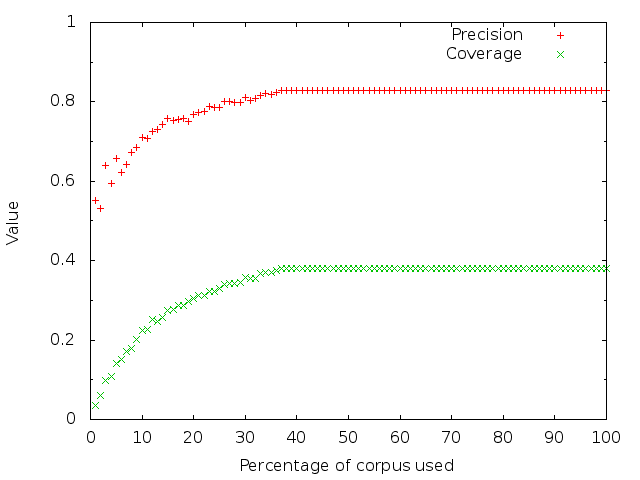
\includegraphics[width=0.45\textwidth]{fig/slot-predicate-percents.png}
    \caption{\label{fig:slot_predicate} slot-predicate model performance when training over a part of the training corpus: from 0 to 100\%.}
\end{figure}

La figure~\ref{fig:slot_predicate} montre que ce niveau de performance ne
demande pas un gros corpus. C'est un enseignement intéressant pour deux
raisons~:

\begin{itemize}

    \item Un corpus de petite taille suffit pour obtenir cette performance, ce
    qui est adapté à des domaines où les corpus même non annotés peuvent être
    petits.

    \item L'algorithme ne fait pas de sur-apprentissage en ayant un biais fort
    et une variance faible, ce qui est souhaitable ici.

\end{itemize}

\subsection{SEMAFOR comparison}

SEMAFOR \citep{das2014frame} est l'état de l'art de l'annotation en rôle
sémantiques supervisée : c'est le système qui obtient les meilleurs résultats
sur le corpus full-text de FrameNet. Toutes les parties du discours sont
annotées alors que nous ne nous concentrons que sur les verbes. Sur la tâche
complète, SEMAFOR obtient un score F1 de XX~\%, score à comparer avec les XX\~
de notre systèmes. Le système de SEMAFOR découpe la tâche en trois parties :

\begin{itemize}
    \item identification des prédicats déclencheurs
    \item identification des frames FrameNet
    \item identification des arguments et annotation en rôles sémantiques 
\end{itemize}

Une comparaison directe n'est pas possible étant donné que les tâches sont
découpées différemment de notre système. Cependant, il est intéressant de noter
l'importance des données d'entraînement : pour l'identification des frames
FrameNet avec des prédicats golds\footnote{les résultats pour des déclencheurs
identifiés manuellement n'ont été donné que pour le corpus SemEval, un
sous-ensemble du corpus FrameNet 1.5 complet}, les mêmes modèles grimpent de
74.21~\% à 90.51~\% quand la taille du corpus augmente en passant du corpus
SemEval (XXX phrases) au corpus FrameNet 1.5 (XXX phrases). De la même manière
pour l'identification des arguments avec des frames FrameNet gold, les
résultats augmente de 48.09~\% 68.83~\%. C'est très encourageant pour les
domaines disposant de très gros corpus, mais suggère que d'autres solutions
sont à identifier pour les domaines où de tels corpus ne sont pas disponibles.

\section{Travaux futurs}

La suite naturelle de ce travail est de l'appliquer à des domaines spécifiques,
ce qui est fait au chapitre~\ref{ch:domainsrl} pour les domaines du football,
du réchauffement climatique et de l'informatique.

Nous pensons aussi prendre en compte la similarité entre les role fillers déjà
identifiés et les role fillers encore à identifier afin d'améliorer nos modèles
de probabilité. En effet, l'information des cadres de sous-catégorisation est
cruciale pour identifier les arguments, mais l'information sémantique
concernant le contenu des role fillers est aussi utile pour déterminer le rôle
correct.
% TODO ref vers chapitre similarité ASFALDA

Enfin, de la même manière que la prise en compte de la voix passive a amélioré
les résultats, d'autres phénomènes de syntaxe profonde doivent être pris en
compte. La coordination est une autre source commune d'erreur.

Quand deux verbes partagent le même sujet, une analyse syntaxique profonde
indique à chaque fois quel est le sujet profond. Voici deux exemples tirés de
notre corpus FrameNet :

\begin{itemize}
    \item You are not fair when you belittle Sheik Bin Baz 's blunder and
          exaggerate the one by Sheik Maqdasi ...
    \item Hostile and even friendly nations routinely steal information from
          U.S. companies and share it with their own companies
\end{itemize}

L'objectif est de traiter ces phénomènes de manière plus générale en intégrant
le système de \cite{ribeyre2013systeme} qui permet de prendre en compte de
nouveaux phénomènes en ajoutant de simple aux règles au système. Ainsi, les
différents phénomènes seront prise en compte de manière cohérente.

\section{Conclusion}

Nous avons implémenté un système d'annotation en rôles sémantiques basé sur la
connaissance. Nous avons utilisé des outils et des corpus disponibles
publiquement qui rendent notre travail facilement reproductible et facilitent
le travail de comparaison, maintenant et dans le futur. Nous avons commencé à
améliorer le système initial, montrant son potentiel. L'indépendance de
l'approche avec le corpus considéré la rendent attractive pour annoter des
domaines ne disposant que de peu ou pas de corpus annotés en rôles sémantiques.
